\documentclass{article}
% \VignettePackage{adegenet-genomics}
% \VignetteIndexEntry{Analysing genome-wide SNP data using adegenet}

\usepackage{graphicx}
\usepackage[colorlinks=true,urlcolor=blue]{hyperref}
\usepackage{array}
\usepackage{color}

\usepackage[utf8]{inputenc} % for UTF-8/single quotes from sQuote()
\newcommand{\code}[1]{{{\tt #1}}}
\title{Analysing genome-wide SNP data using  \textit{adegenet} 1.3-0}
\author{Thibaut Jombart}
\date{\today}




\sloppy
\hyphenpenalty 10000


\usepackage{Sweave}
\begin{document}





\definecolor{Soutput}{rgb}{0,0,0.56}
\definecolor{Sinput}{rgb}{0.56,0,0}
\DefineVerbatimEnvironment{Sinput}{Verbatim}
{formatcom={\color{Sinput}},fontsize=\footnotesize, baselinestretch=0.75}
\DefineVerbatimEnvironment{Soutput}{Verbatim}
{formatcom={\color{Soutput}},fontsize=\footnotesize, baselinestretch=0.75}

\color{black}

\maketitle

\begin{abstract}
  Genome-wide SNP data can quickly be challenging to analyse using standard
  computer. The package \textit{adegenet} \cite{tjart05} for the R software \cite{np145}
  implements representation of these data with unprecedented efficiency
  using the classes \texttt{SNPbin} and \texttt{genlight}, which can require up to 60 times less RAM than usual
  representation using allele frequencies.
  This vignette introduces these classes and illustrates how these objects can be handled and
  analyzed in R.
  %% It also introduces more advanced features of an API in C language which may be useful to develop
  %% new method based on these objects.
\end{abstract}

\newpage

\tableofcontents


\newpage
%%%%%%%%%%%%%%%%
%%%%%%%%%%%%%%%%
\section{Introduction}
%%%%%%%%%%%%%%%%
%%%%%%%%%%%%%%%%
Modern sequencing technologies now make complete genomes more widely accessible.
The subsequent amounts of genetic data pose challenges in terms of storing and handling the data,
making former tools developed for classical genetic markers such as microsatellite impracticable using
standard computers.
Adegenet has developed new object classes dedicated to handling genome-wide polymorphism (SNPs) with
minimum rapid access memory (RAM) requirements.
\\

Two new formal classes have been implemented: \texttt{SNPbin}, used to store genome-wide SNPs for
one individual, and \texttt{genlight}, which stored the same information for multiple individuals.
Information represented this way is binary: only biallelic SNPs can be stored and analyzed using these classes.
However, these objects are otherwise very flexible, and can incorporate different levels of ploidy
across individuals within a single dataset.
In this vignette, we present these object classes and show how their content can be further handled and
content analyzed.





%%%%%%%%%%%%%%%%
%%%%%%%%%%%%%%%%
\section{Classes of objects}
%%%%%%%%%%%%%%%%
%%%%%%%%%%%%%%%%

%%%%%%%%%%%%%%%%
\subsection{\code{SNPbin}: storage of single genomes}
%%%%%%%%%%%%%%%%
The class \texttt{SNPbin} is the core representation of biallelic SNPs which allows to represent
data with unprecedented efficiency.
The essential idea is to code binary SNPs not as integers, but as bits. This operation is tricky in
R as there is no handling of bits, only bytes -- series of 8 bits. However, the class
\texttt{SNPbin} handles this transparently using sub-rountines in C language.
Considerable efforts have been made so that the user does not have to dig into the complex internal
structure of the objects, and can handle \texttt{SNPbin} objects as easily as possible.
\\

Like \texttt{genind} and \texttt{genpop} objects, \texttt{SNPbin} is a formal "S4" class. The
structure of these objects is detailed in the dedicated manpage (\texttt{?SNPbin}). As all S4
objects, instances of the class \texttt{SNPbin} are composed of slots accessible using the
\texttt{@} operator. This content is generic (it is the same for all instances of the class), and returned by:
\begin{Schunk}
\begin{Sinput}
> library(adegenet)
> getClassDef("SNPbin")
\end{Sinput}
\begin{Soutput}
Class "SNPbin" [package "adegenet"]

Slots:
                                                             
Name:         snp      n.loc    NA.posi      label     ploidy
Class:       list    integer    integer charOrNULL    integer
\end{Soutput}
\end{Schunk}

The slots respectively contain:
\begin{itemize}
  \item \texttt{snp}: SNP data with specific internal coding.
  \item \texttt{n.loc}: the number of SNPs stored in the object.
  \item \texttt{NA.posi}: position of the missing data (NAs).
  \item \texttt{label}: an optional label for the individual.
  \item \texttt{ploidy}: the ploidy level of the genome.
\end{itemize}

New objects are created using \texttt{new}, with these slots as arguments.
If no argument is provided, an empty object is created:
\begin{Schunk}
\begin{Sinput}
> new("SNPbin")
\end{Sinput}
\begin{Soutput}
 === S4 class SNPbin ===
 0 SNPs coded as bits
 Ploidy: 1
 0 (NaN %) missing data
\end{Soutput}
\end{Schunk}
In practice, only the \texttt{snp} information and possibly the ploidy has to be provided; various
formats are accepted for the \texttt{snp} component, but the simplest is a vector of integers (or
numeric) indicating the number of second allele at each locus.
The argument \texttt{snp}, if provided alone, does not have to be named:
\begin{Schunk}
\begin{Sinput}
> x <- new("SNPbin", c(0, 1, 1, 2, 0, 0, 1))
> x
\end{Sinput}
\begin{Soutput}
 === S4 class SNPbin ===
 7 SNPs coded as bits
 Ploidy: 2
 0 (0 %) missing data
\end{Soutput}
\end{Schunk}

If not provided, the ploidy is detected from the data and determined as the largest number in the
input vector. Obviously, in many cases this will not be adequate, but ploidy can always be rectified
afterwards; for instance:
\begin{Schunk}
\begin{Sinput}
> x
\end{Sinput}
\begin{Soutput}
 === S4 class SNPbin ===
 7 SNPs coded as bits
 Ploidy: 2
 0 (0 %) missing data
\end{Soutput}
\begin{Sinput}
> ploidy(x) <- 3
> x
\end{Sinput}
\begin{Soutput}
 === S4 class SNPbin ===
 7 SNPs coded as bits
 Ploidy: 3
 0 (0 %) missing data
\end{Soutput}
\end{Schunk}

\noindent The internal coding of the objects is cryptic, and not meant to be accessed directly:
\begin{Schunk}
\begin{Sinput}
> x@snp
\end{Sinput}
\begin{Soutput}
[[1]]
[1] 08

[[2]]
[1] 4e
\end{Soutput}
\end{Schunk}
Fortunately, data are easily converted back into integers:
\begin{Schunk}
\begin{Sinput}
> as.integer(x)
\end{Sinput}
\begin{Soutput}
[1] 0 1 1 2 0 0 1
\end{Soutput}
\end{Schunk}

~\\

The main interest of this representation is its efficiency in terms of storage.
For instance:
\begin{Schunk}
\begin{Sinput}
> dat <- sample(0:1, 1e+06, replace = TRUE)
> print(object.size(dat), unit = "auto")
\end{Sinput}
\begin{Soutput}
3.8 Mb
\end{Soutput}
\begin{Sinput}
> x <- new("SNPbin", dat)
> print(object.size(x), unit = "auto")
\end{Sinput}
\begin{Soutput}
123.4 Kb
\end{Soutput}
\end{Schunk}
here, we converted a million SNPs into a \texttt{SNPbin} object, which turns out to be
32 smaller than the original data.
However, the information in \texttt{dat} and \texttt{x} is strictly identical:
\begin{Schunk}
\begin{Sinput}
> identical(as.integer(x), dat)
\end{Sinput}
\begin{Soutput}
[1] TRUE
\end{Soutput}
\end{Schunk}
The advantage of this storage is therefore being extremely compact, and allowing to analyse big
datasets using standard computers.
%% Obviously, usual computations demand data to be at one moment coded as numeric values (as opposed to bits).
%% However in most cases, we can proceed by only converting one or two genomes back to numeric values
%% at a time, therefore keeping RAM requirements low, albeit at a possible increase in computational time.
%% This however is minimized by two ways: i) conversion routines are optimized for speed using C code
%% ii) smaller objects are handled, therefore decreasing the possibly high computational time taken by memory allocation.
\\

While \texttt{SNPbin} objects are the very mean by which we store data efficiently, in practice
we need to analyze several genomes at a time.
This is made possible by the class \texttt{genlight}, which relies on \texttt{SNPbin} but allows for
storing data from several genomes at a time.




%%%%%%%%%%%%%%%%
\subsection{\code{genlight}: storage of multiple genomes}
%%%%%%%%%%%%%%%%

Like \texttt{SNPbin}, \texttt{genlight} is a formal S4 class.
The slots of instances of this class are described by:
\begin{Schunk}
\begin{Sinput}
> getClassDef("genlight")
\end{Sinput}
\begin{Soutput}
Class "genlight" [package "adegenet"]

Slots:
                                                                       
Name:           gen        n.loc    ind.names    loc.names      loc.all
Class:         list      integer   charOrNULL   charOrNULL   charOrNULL
                                                                       
Name:    chromosome     position       ploidy          pop        other
Class: factorOrNULL    intOrNULL    intOrNULL factorOrNULL         list
\end{Soutput}
\end{Schunk}
As it can be seen, these objects allow for storing more information in addition to vectors of SNP frequencies.
More precisely, their content is (see \texttt{?genlight} for more details):
\begin{itemize}
  \item \texttt{gen}: SNP data for different individuals, each stored as a \texttt{SNPbin}; loci
    have to be identical across all individuals.
  \item \texttt{n.loc}: the number of SNPs stored in the object.
  \item \texttt{ind.names}: (optional) labels for the individuals.
  \item \texttt{loc.names}: (optional) labels for the loci.
  \item \texttt{loc.all}: (optional) alleles of the loci separated by '/' (e.g. 'a/t', 'g/c', etc.).
  \item \texttt{chromosome}: (optional) a factor indicating the chromosome to which the SNPs belong.
  \item \texttt{position}: (optional) the position of each SNPs in their chromosome.
  \item \texttt{ploidy}: (optional) the ploidy of each individual.
  \item \texttt{pop}: (optional) a factor grouping individuals into 'populations'.
  \item \texttt{other}: (optional) a list containing any supplementary information to be stored with
    the data.
\end{itemize}

\noindent Like \texttt{SNPbin} object, \texttt{genlight} object are created using the constructor \texttt{new},
providing content for the slots above as arguments.
When none is provided, an empty object is created:
\begin{Schunk}
\begin{Sinput}
> new("genlight")
\end{Sinput}
\begin{Soutput}
 === S4 class genlight ===
 0 genotypes,  0 binary SNPs
\end{Soutput}
\end{Schunk}
The most important information to provide is obviously the genotypes (argument \texttt{gen}); these
can be provided as:
\begin{itemize}
\item a \texttt{list} of integer vectors representing the number of second allele at each locus.
\item a \texttt{matrix} / \texttt{data.frame} of integers, with individuals in rows and SNPs in columns.
\item a list of \texttt{SNPbin} objects.
\end{itemize}

Ploidy has to be consistent across loci for a given individual, but individuals do not have to have
the same ploidy, so that it is possible to have hapoid,
diploid, and tetraploid individuals in the same dataset; for instance:
\begin{Schunk}
\begin{Sinput}
> x <- new("genlight", list(indiv1 = c(1, 1, 0, 1, 1, 0), indiv2 = c(2, 
+     1, 1, 0, 0, 0), toto = c(2, 2, 0, 0, 4, 4)))
> x
\end{Sinput}
\begin{Soutput}
 === S4 class genlight ===
 3 genotypes,  6 binary SNPs
 Ploidy statistics (min/median/max): 1 / 2 / 4
 0 (0 %) missing data
\end{Soutput}
\begin{Sinput}
> ploidy(x)
\end{Sinput}
\begin{Soutput}
indiv1 indiv2   toto 
     1      2      4 
\end{Soutput}
\end{Schunk}

As for \texttt{SNPbin}, \texttt{genlight} objects can be converted back to integers vectors, stored
as matrices or lists:
\begin{Schunk}
\begin{Sinput}
> as.list(x)
\end{Sinput}
\begin{Soutput}
$indiv1
[1] 1 1 0 1 1 0

$indiv2
[1] 2 1 1 0 0 0

$toto
[1] 2 2 0 0 4 4
\end{Soutput}
\begin{Sinput}
> as.matrix(x)
\end{Sinput}
\begin{Soutput}
       [,1] [,2] [,3] [,4] [,5] [,6]
indiv1    1    1    0    1    1    0
indiv2    2    1    1    0    0    0
toto      2    2    0    0    4    4
\end{Soutput}
\end{Schunk}

\noindent In practice, \texttt{genlight} objects can be handled as if they were matrices of integers
as the one above returned by \texttt{as.matrix}.
However, they offer the advantage of efficient storage of the information; for instance, we can
simulate 50 individuals typed for 1,00,000 SNPs each (including occasional NAs):
\begin{Schunk}
\begin{Sinput}
> dat <- lapply(1:50, function(i) sample(c(0, 1, NA), 1e+06, prob = c(0.5, 
+     0.499, 0.001), replace = TRUE))
> names(dat) <- paste("indiv", 1:length(dat))
> print(object.size(dat), unit = "auto")
\end{Sinput}
\begin{Soutput}
381.5 Mb
\end{Soutput}
\begin{Sinput}
> x <- new("genlight", dat)
> print(object.size(x), unit = "auto")
\end{Sinput}
\begin{Soutput}
6.2 Mb
\end{Soutput}
\begin{Sinput}
> object.size(dat)/object.size(x)
\end{Sinput}
\begin{Soutput}
61.3318323604199 bytes
\end{Soutput}
\end{Schunk}
here again, the storage if the data is much more efficient in \texttt{genlight} than using integers: converted data occupy
61 times less memory than the original data.
\\

The advantage of this storage is therefore being extremely compact, and allowing to analyse very large
datasets using standard computers.
Obviously, usual computations demand data to be at one moment coded as numeric values (as opposed to bits).
However, most usual computations can be achieved by only converting one or two genomes back to numeric values
at a time, therefore keeping RAM requirements low, albeit at a possible cost of increased computational time.
This however is minimized by three ways:
\begin{enumerate}
\item conversion routines are optimized for speed using C code.
\item using parallel computation where multicore architectures are available.
\item handling smaller objects, thereby decreasing the possibly high computational time taken by memory allocation.
\end{enumerate}

While this makes implementing methods more complicated.
In practice, routines are implemented so as to minimize
the amount of data converted back to integers, use C code where possible, and use multiple cores
if the package \textit{multicore} is installed an multiple cores are available.
Fortunately, these underlying technical issues are oblivious to the user, and one merely needs to
know how to manipulate \texttt{genlight} objects using a few key functions to be able to analyze data.






%%%%%%%%%%%%%%%%
%%%%%%%%%%%%%%%%
\section{Data handling using \texttt{genlight} objects}
%%%%%%%%%%%%%%%%
%%%%%%%%%%%%%%%%

%%%%%%%%%%%%%%%%
\subsection{Using accessors}
%%%%%%%%%%%%%%%%

In the following, we demonstrate how to manipulate and analyse \texttt{genlight} objects.
The phylosophy underlying formal (S4) classes in general, and \texttt{genlight} objects in
particular, is that internal representation of the information can be complex as long as accessing
this information is simple.
This is made possible by decoupling storage and accession: the user is not meant to access the
content of the object directly, but has to use \texttt{accessors} to retrieve or modify information.
\\

Available accessors are documented in \code{?genlight}.
Most of them are identical to accessors for \texttt{genind} and \texttt{genpop} objects, such as:
\begin{itemize}
  \item \texttt{nInd}: returns the number of individuals in the object.
  \item \texttt{nLoc}: returns the number of loci (SNPs).
  \item \texttt{indNames}$^{\dagger}$: returns/sets labels for individuals.
  \item \texttt{locNames}$^{\dagger}$: returns/sets labels for loci (SNPs).
  \item \texttt{alleles}$^{\dagger}$: returns/sets alleles.
  \item \texttt{ploidy}$^{\dagger}$: returns/sets ploidy of the individuals.
  \item \texttt{pop}$^{\dagger}$: returns/sets a factor grouping individuals.
  \item \texttt{other}$^{\dagger}$: returns/sets misc information stored as a list.
\end{itemize}
where $^{\dagger}$ indicates that a replacement method is available using \texttt{<-}; for instance:
\begin{Schunk}
\begin{Sinput}
> dat <- lapply(1:3, function(i) sample(0:2, 10, replace = TRUE))
> dat
\end{Sinput}
\begin{Soutput}
[[1]]
 [1] 2 0 0 1 1 0 2 2 2 2

[[2]]
 [1] 0 1 1 2 0 1 2 0 1 0

[[3]]
 [1] 1 2 0 2 2 1 2 2 0 1
\end{Soutput}
\begin{Sinput}
> x <- new("genlight", dat)
> x
\end{Sinput}
\begin{Soutput}
 === S4 class genlight ===
 3 genotypes,  10 binary SNPs
 Ploidy: 2
 0 (0 %) missing data
\end{Soutput}
\begin{Sinput}
> indNames(x)
\end{Sinput}
\begin{Soutput}
NULL
\end{Soutput}
\begin{Sinput}
> indNames(x) <- paste("individual", 1:3)
> indNames(x)
\end{Sinput}
\begin{Soutput}
[1] "individual 1" "individual 2" "individual 3"
\end{Soutput}
\begin{Sinput}
> locNames(x)
> locNames(x) <- paste("SNP", 1:nLoc(x), sep = ".")
> as.matrix(x)
\end{Sinput}
\begin{Soutput}
             SNP.1 SNP.2 SNP.3 SNP.4 SNP.5 SNP.6 SNP.7 SNP.8 SNP.9 SNP.10
individual 1     2     0     0     1     1     0     2     2     2      2
individual 2     0     1     1     2     0     1     2     0     1      0
individual 3     1     2     0     2     2     1     2     2     0      1
\end{Soutput}
\end{Schunk}

\noindent
In addition, some specific accessors are available for \texttt{genlight} objects:
\begin{itemize}
  \item \texttt{NA.posi}: returns the position of missing values in each individual.
  \item \texttt{chromosome}$^{\dagger}$: returns/sets the chromosome of each SNP.
  \item \texttt{chr}$^{\dagger}$: same as \texttt{chromosome} --- used as a shortcut.
  \item \texttt{position}$^{\dagger}$: returns/sets the position of each SNP.
\end{itemize}


Accessors are meant to be clever about replacement, meaning that they try hard to prevent
replacement with inconsistent values. For instance, in object \texttt{x}:
\begin{Schunk}
\begin{Sinput}
> x
\end{Sinput}
\begin{Soutput}
 === S4 class genlight ===
 3 genotypes,  10 binary SNPs
 Ploidy: 2
 0 (0 %) missing data
 @loc.names: labels of the SNPs
\end{Soutput}
\end{Schunk}
if we try to set information about the chromosomes of the SNPs, the instruction:
\begin{Schunk}
\begin{Sinput}
> chr(x) <- rep("chr-1", 7)
\end{Sinput}
\end{Schunk}
will generate an error because the provided factor does not match the number of loci (10), while:
\begin{Schunk}
\begin{Sinput}
> chr(x) <- rep("chr-1", 10)
> x
\end{Sinput}
\begin{Soutput}
 === S4 class genlight ===
 3 genotypes,  10 binary SNPs
 Ploidy: 2
 0 (0 %) missing data
 @chromosome: chromosome of the SNPs
 @loc.names: labels of the SNPs
\end{Soutput}
\begin{Sinput}
> chr(x)
\end{Sinput}
\begin{Soutput}
 [1] chr-1 chr-1 chr-1 chr-1 chr-1 chr-1 chr-1 chr-1 chr-1 chr-1
Levels: chr-1
\end{Soutput}
\end{Schunk}
is a valid replacement.




%%%%%%%%%%%%%%%%
\subsection{Subsetting the data}
%%%%%%%%%%%%%%%%
\texttt{genlight} objects are meant to be handled as if they were matrices of allele numbers, as
returned by \texttt{as.matrix}.
Therefore, subsetting can be achieved using $[$ \texttt{idx.row , idx.col} $]$ where \texttt{idx.row}
and \texttt{idx.col} are indices for rows (individuals) and columns (SNPs).
For instance, using the previous toy dataset, we try a few classical subsetting of rows and columns:
\begin{Schunk}
\begin{Sinput}
> x
\end{Sinput}
\begin{Soutput}
 === S4 class genlight ===
 3 genotypes,  10 binary SNPs
 Ploidy: 2
 0 (0 %) missing data
 @chromosome: chromosome of the SNPs
 @loc.names: labels of the SNPs
\end{Soutput}
\begin{Sinput}
> as.matrix(x)
\end{Sinput}
\begin{Soutput}
             SNP.1 SNP.2 SNP.3 SNP.4 SNP.5 SNP.6 SNP.7 SNP.8 SNP.9 SNP.10
individual 1     2     0     0     1     1     0     2     2     2      2
individual 2     0     1     1     2     0     1     2     0     1      0
individual 3     1     2     0     2     2     1     2     2     0      1
\end{Soutput}
\begin{Sinput}
> as.matrix(x[c(1, 3), ])
\end{Sinput}
\begin{Soutput}
             SNP.1 SNP.2 SNP.3 SNP.4 SNP.5 SNP.6 SNP.7 SNP.8 SNP.9 SNP.10
individual 1     2     0     0     1     1     0     2     2     2      2
individual 3     1     2     0     2     2     1     2     2     0      1
\end{Soutput}
\begin{Sinput}
> as.matrix(x[, c(TRUE, FALSE)])
\end{Sinput}
\begin{Soutput}
             SNP.1 SNP.3 SNP.5 SNP.7 SNP.9
individual 1     2     0     1     2     2
individual 2     0     1     0     2     1
individual 3     1     0     2     2     0
\end{Soutput}
\begin{Sinput}
> as.matrix(x[1:2, c(1, 1, 1, 2, 2, 2, 3, 3, 3)])
\end{Sinput}
\begin{Soutput}
             SNP.1 SNP.1 SNP.1 SNP.2 SNP.2 SNP.2 SNP.3 SNP.3 SNP.3
individual 1     2     2     2     0     0     0     0     0     0
individual 2     0     0     0     1     1     1     1     1     1
\end{Soutput}
\end{Schunk}


Moreover, one can split data into blocks of SNPs using \texttt{seploc}.
This can be achieved by specifying either a number of blocks (argument \texttt{n.block}) or the size
of the blocks (argument \texttt{block.size}). The function also allows for randomizing the
distribution of the SNPs in the blocks (argument \texttt{random=TRUE}), which is especially useful
to replace computations that cannot be achieved on the whole dataset with parallelized computations performed on random blocks.
For instance:
\begin{Schunk}
\begin{Sinput}
> x
\end{Sinput}
\begin{Soutput}
 === S4 class genlight ===
 3 genotypes,  10 binary SNPs
 Ploidy: 2
 0 (0 %) missing data
 @chromosome: chromosome of the SNPs
 @loc.names: labels of the SNPs
\end{Soutput}
\begin{Sinput}
> as.matrix(x)
\end{Sinput}
\begin{Soutput}
             SNP.1 SNP.2 SNP.3 SNP.4 SNP.5 SNP.6 SNP.7 SNP.8 SNP.9 SNP.10
individual 1     2     0     0     1     1     0     2     2     2      2
individual 2     0     1     1     2     0     1     2     0     1      0
individual 3     1     2     0     2     2     1     2     2     0      1
\end{Soutput}
\begin{Sinput}
> seploc(x, n.block = 2)
\end{Sinput}
\begin{Soutput}
$block.1
 === S4 class genlight ===
 3 genotypes,  5 binary SNPs
 Ploidy: 2
 0 (0 %) missing data
 @chromosome: chromosome of the SNPs
 @loc.names: labels of the SNPs

$block.2
 === S4 class genlight ===
 3 genotypes,  5 binary SNPs
 Ploidy: 2
 0 (0 %) missing data
 @chromosome: chromosome of the SNPs
 @loc.names: labels of the SNPs
\end{Soutput}
\begin{Sinput}
> lapply(seploc(x, n.block = 2), as.matrix)
\end{Sinput}
\begin{Soutput}
$block.1
             SNP.1 SNP.2 SNP.3 SNP.4 SNP.5
individual 1     2     0     0     1     1
individual 2     0     1     1     2     0
individual 3     1     2     0     2     2

$block.2
             SNP.6 SNP.7 SNP.8 SNP.9 SNP.10
individual 1     0     2     2     2      2
individual 2     1     2     0     1      0
individual 3     1     2     2     0      1
\end{Soutput}
\end{Schunk}
splits the data into two blocks of contiguous SNPs, while:
\begin{Schunk}
\begin{Sinput}
> lapply(seploc(x, n.block = 2, random = TRUE), as.matrix)
\end{Sinput}
\begin{Soutput}
$block.1
             SNP.1 SNP.8 SNP.4 SNP.2 SNP.6
individual 1     2     2     1     0     0
individual 2     0     0     2     1     1
individual 3     1     2     2     2     1

$block.2
             SNP.7 SNP.10 SNP.3 SNP.9 SNP.5
individual 1     2      2     0     2     1
individual 2     2      0     1     1     0
individual 3     2      1     0     0     2
\end{Soutput}
\end{Schunk}
generates blocks of randomly selected SNPs.




%%%%%%%%%%%%%%%%
\subsection{Data conversions}
%%%%%%%%%%%%%%%%

% % % % % % % % % % % % %
\subsubsection{The \texttt{.snp} format}
% % % % % % % % % % % % %

\textit{adegenet} has defined its own format for storing biallelic SNP data in text files with
extension \texttt{.snp}.
This format has several advantages: it is fairly compact (more so than usual non-compressed
formats), allows for any information about individuals or loci to be stored, allows for comments,
and is easily parsed --- in particular, not all information has to be read at a time, again
minimizing RAM requirements for import procedures.


An example file of this format is distributed with adegenet.
Once the package has been installed, the file can be accessed by typing:
\begin{Schunk}
\begin{Sinput}
> file.show(system.file("files/exampleSnpDat.snp", package = "adegenet"))
\end{Sinput}
\end{Schunk}
Otherwise, this file is also accessible from the \textit{adegenet} website (section 'Documents').
A complete description of the \texttt{.snp} format is provided in the comment section of the file.
\\


The structure of a \texttt{.snp} file can be summarized as follows:
\begin{itemize}
\item a (possibly empty) \texttt{comment section}
\item \texttt{meta-information}, i.e. information about loci or individuals, stored as named vectors
\item \texttt{genotypes}, stored as named vectors
\end{itemize}

The \textit{comment section} can starts with the line:\\
\begin{verbatim}
>>>> begin comments - do not remove this line <<<<
\end{verbatim}
\noindent and ends with the line:\\
\begin{verbatim}
>>>> end comments - do not remove this line <<<<}
\end{verbatim}
\noindent While this section can be left empty, these two lines have to be present for the format to
be valid.
Each \textit{meta-information} is stored using two lines, the first starting as:
\begin{verbatim}
>> name-of-the-information
\end{verbatim}
and the second containing the information itself, each item separated by a single space.
Any label can be used, but some specific names will be recognized and interpreted by the parser:
\begin{itemize}
\item \texttt{position}: the following line contains integers giving the position of the SNPs on the sequence
\item \texttt{allele}: character strings representing the two alleles of each loci separated by "/"
\item \texttt{population}: character strings indicating a group memberships of the individuals
\item \texttt{ploidy}: integers indicating the ploidy of each individual; alternatively, one single integer if
all individuals have the same ploidy
\item \texttt{chromosome}: character strings indicating the chromosome on which the SNP are located
\end{itemize}
Each \textit{genotype} is stored using two lines, the first being:
\begin{verbatim}
> label-of-the-individual
\end{verbatim}
and the second being integers corresponding to the number of
second allele for each loci, without separators; missing data are coded as '\texttt{-}'.
\\


\texttt{.snp} files can be read in R using \texttt{read.snp}, which converts data into
\texttt{genlight} objects.
The function reads data by chunks of a several individuals (minimum 1, no maximum besides RAM
constraints) at a time, which allows one to read massive datasets with negligible RAM requirements
(albeit at a cost of computational time). The argument \texttt{chunkSize} indicates the number of
genomes read at a time; larger values mean reading data faster but require more RAM.
We can illustrate \texttt{read.snp} using the example file mentioned above.
The non-comment part of the file reads:
\begin{verbatim}
[...]
>> position
1 8 11 43
>> allele
a/t g/c a/c t/a
>> population
Brit Brit Fren monster NA
>> ploidy
2
> foo
1020
> bar
0012
> toto
10-0
> Nyarlathotep
0120
> an even longer label but OK since on a single line
1100
\end{verbatim}
We read the file in using:
\begin{Schunk}
\begin{Sinput}
> obj <- read.snp(system.file("files/exampleSnpDat.snp", package = "adegenet"), 
+     chunk = 2)
\end{Sinput}
\begin{Soutput}
 Reading biallelic SNP data file into a genlight object... 


 Reading comments... 

 Reading general information... 

 Reading 5 genotypes... 
...
 Checking consistency... 

 Building final object... 

...done.
\end{Soutput}
\begin{Sinput}
> obj
\end{Sinput}
\begin{Soutput}
 === S4 class genlight ===
 5 genotypes,  4 binary SNPs
 Ploidy: 2
 1 (0.05 %) missing data
 @pop: individual membership for 4 populations
 @position: position of the SNPs
 @alleles: alleles of the SNPs
\end{Soutput}
\begin{Sinput}
> as.matrix(obj)
\end{Sinput}
\begin{Soutput}
                                                   1.a/t 8.g/c 11.a/c 43.t/a
foo                                                    1     0      2      0
bar                                                    0     0      1      2
toto                                                   1     0     NA      0
Nyarlathotep                                           0     1      2      0
an even longer label but OK since on a single line     1     1      0      0
\end{Soutput}
\begin{Sinput}
> alleles(obj)
\end{Sinput}
\begin{Soutput}
[1] "a/t" "g/c" "a/c" "t/a"
\end{Soutput}
\begin{Sinput}
> pop(obj)
\end{Sinput}
\begin{Soutput}
[1] Brit    Brit    Fren    monster NA     
Levels: Brit Fren monster NA
\end{Soutput}
\begin{Sinput}
> indNames(obj)
\end{Sinput}
\begin{Soutput}
[1] "foo"                                               
[2] "bar"                                               
[3] "toto"                                              
[4] "Nyarlathotep"                                      
[5] "an even longer label but OK since on a single line"
\end{Soutput}
\end{Schunk}
Note that \texttt{system.file} is generally useless: it is only used in this example to access a
file installed alongside the package. Usual calls to \texttt{read.snp} will ressemble:
\begin{Schunk}
\begin{Sinput}
> obj <- read.snp("path-to-my-file.snp")
\end{Sinput}
\end{Schunk}


% % % % % % % % % % % % %
\subsubsection{Importing data from PLINK}
% % % % % % % % % % % % %

Genome-wide SNP data of diploid organisms are frequently analyzed using PLINK, whose format is
therefore becoming a standard.
Data with PLINK format (\texttt{.raw}) can be imported into \texttt{genlight} objects using \texttt{read.PLINK}.
This function requires the data to be saved in PLINK using the `\textit{-recodeA}` option (see details
section in \texttt{?read.PLINK}).
More information on exporting from PLINK can be found at \url{http://pngu.mgh.harvard.edu/~purcell/plink/dataman.shtml#recode}.
\\


Like \texttt{read.snp}, \texttt{read.PLINK} has the advantage of reading data by chunks of a few individuals
(down to a single one at a time, no upper limits), which minimizes the amount of memory needed to read information
before its conversion to \texttt{genlight}; however, using more chunks also means more computational
time, since the procedure has to re-read the same file several time.
Note that meta information about the loci also known as \texttt{.map} can also be read alongside a
\texttt{.raw} file using the argument \texttt{map.file}.
Alternatively, such information can be added to a \texttt{genlight} object afterwards using \texttt{extract.PLINKmap}.





% % % % % % % % % % % % %
\subsubsection{Extracting SNPs from alignments}
% % % % % % % % % % % % %
In many cases, raw genomic data are available as aligned sequences, in which case extracting
polymorphic sites can be non-trivial.
The biggest issue is again memory: most software extracting SNPs from aligned sequences
require all the sequences to be stored in memory at a time, a duty that most common computers cannot undertake.
\textit{adegenet} implements a more parsimonious alternative which allows for extracting SNPs from
alignment while processing a reduced number of sequences (down to a single) at a time.
\\

The function \texttt{fasta2genlight} extracts SNPs from alignments with \textit{fasta} format (file
extensions '\texttt{.fasta}', '\texttt{.fas}', or '\texttt{.fa}').
Like \texttt{read.snp} and \texttt{read.PLINK}, \texttt{fasta2genlight} processes data by chunks of
individuals so as to save memory requirements.
It first scans the whole file for polymorphic positions, and then extracts all biallelic SNPs from
the alignment.
\\

\texttt{fasta2genlight} is illustrated like \texttt{read.snp} using a toy dataset distributed
alongside the package.
The file is first located using \texttt{system.file}, and then processed using \texttt{fasta2genlight}:
\begin{Schunk}
\begin{Sinput}
> myPath <- system.file("files/usflu.fasta", package = "adegenet")
> flu <- fasta2genlight(myPath, chunk = 10)
\end{Sinput}
\begin{Soutput}
 Converting FASTA alignment into a genlight object... 


 Looking for polymorphic positions... 
........................................................................................................................................................................................................................................................................................................................................................................
 Extracting SNPs from the alignment... 
........................................................................................................................................................................................................................................................................................................................................................................
 Building final object... 

...done.
\end{Soutput}
\begin{Sinput}
> flu
\end{Sinput}
\begin{Soutput}
 === S4 class genlight ===
 80 genotypes,  274 binary SNPs
 Ploidy: 1
 26 (0 %) missing data
 @position: position of the SNPs
 @alleles: alleles of the SNPs
\end{Soutput}
\end{Schunk}

\noindent \texttt{flu} is a \texttt{genlight} object containing SNPs of 80 isolates of seasonal
influenza (H3N2) sampled within the US over the last two decades; sequences correspond to the
hemagglutinin (HA) segment.
Besides genotypes, \texttt{flu} contains the positions of the SNPs and the alleles at each retained loci.
Names of the loci are constructed as the combination of both:
\begin{Schunk}
\begin{Sinput}
> head(position(flu), 20)
\end{Sinput}
\begin{Soutput}
 [1]   7  12  31  32  36  37  44  45  52  60  62  72  73  78  96  99 105 108 121
[20] 128
\end{Soutput}
\begin{Sinput}
> head(alleles(flu), 20)
\end{Sinput}
\begin{Soutput}
 [1] "a/g" "c/t" "t/c" "t/c" "t/c" "c/a" "t/c" "c/t" "a/g" "c/t" "g/t" "c/a"
[13] "a/g" "a/g" "a/g" "c/t" "a/g" "g/a" "c/a" "a/g"
\end{Soutput}
\begin{Sinput}
> head(locNames(flu), 20)
\end{Sinput}
\begin{Soutput}
 [1] "7.a/g"   "12.c/t"  "31.t/c"  "32.t/c"  "36.t/c"  "37.c/a"  "44.t/c" 
 [8] "45.c/t"  "52.a/g"  "60.c/t"  "62.g/t"  "72.c/a"  "73.a/g"  "78.a/g" 
[15] "96.a/g"  "99.c/t"  "105.a/g" "108.g/a" "121.c/a" "128.a/g"
\end{Soutput}
\end{Schunk}

\noindent It is usually informative to assess the position of the polymorphic sites within the
genome; this is very easily done in R, using \texttt{density} with an appropriate bandewidth:
\begin{Schunk}
\begin{Sinput}
> temp <- density(position(flu), bw = 10)
> plot(temp, type = "n", xlab = "Position in the alignment", main = "Location of the SNPs", 
+     xlim = c(0, 1701))
> polygon(c(temp$x, rev(temp$x)), c(temp$y, rep(0, length(temp$x))), 
+     col = transp("blue", 0.3))
> points(position(flu), rep(0, nLoc(flu)), pch = "|", col = "blue")
\end{Sinput}
\end{Schunk}
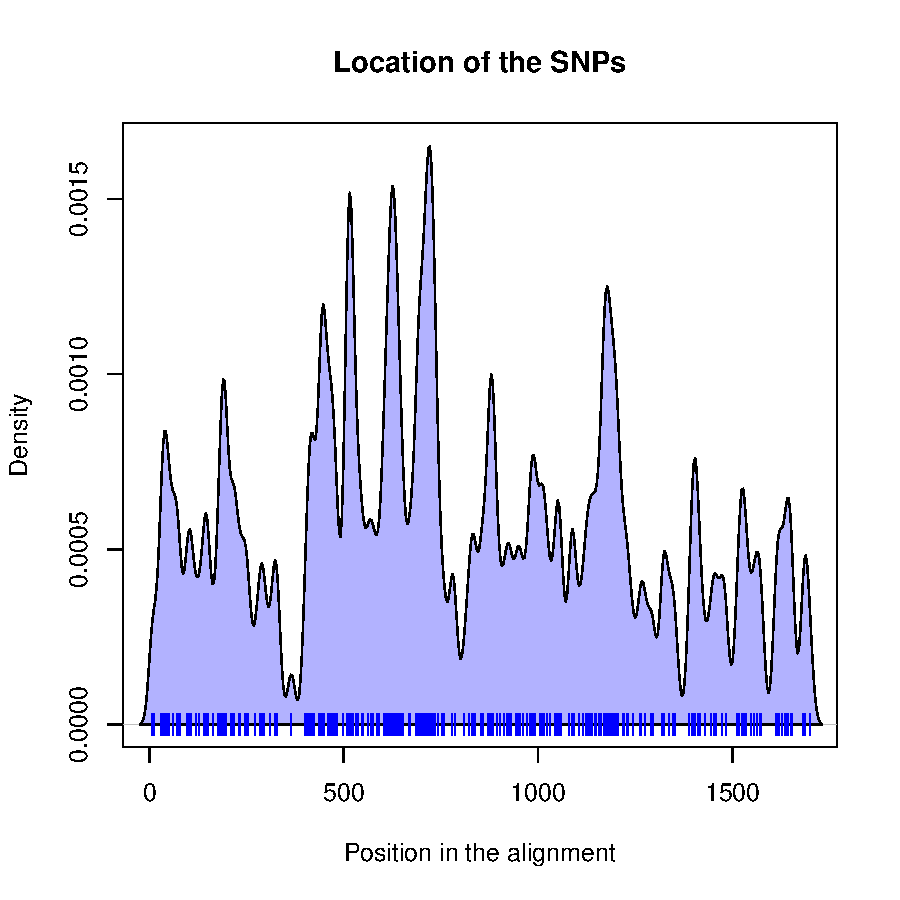
\includegraphics{figs/genomics-027}

\noindent In this case, SNPs are distributed fairly homogeneously across the HA segment, with
a few possible hotspots of polymorphism within positions 400---700.
\\


Note that retaining only biallelic sites may cause minor loss of information, as sites
with more than 2 alleles are discarded from the data.
It is however possible to ask \texttt{fasta2genlight} to keep track of the number of alleles for
each site of the original alignment, by specifying:
\begin{Schunk}
\begin{Sinput}
> flu <- fasta2genlight(myPath, chunk = 10, saveNbAlleles = TRUE, 
+     quiet = TRUE)
> flu
\end{Sinput}
\begin{Soutput}
 === S4 class genlight ===
 80 genotypes,  274 binary SNPs
 Ploidy: 1
 26 (0 %) missing data
 @position: position of the SNPs
 @alleles: alleles of the SNPs
 @other: a list containing: nb.all.per.loc 
\end{Soutput}
\end{Schunk}

\noindent The output object \texttt{flu} now contains the number of alleles of each position, stored
in the \texttt{other} slot:
\begin{Schunk}
\begin{Sinput}
> head(other(flu)$nb.all.per.loc, 20)
\end{Sinput}
\begin{Soutput}
 [1] 1 1 1 1 1 1 2 1 1 1 1 2 1 1 1 1 1 1 1 1
\end{Soutput}
\begin{Sinput}
> 100 * mean(unlist(other(flu)) > 1)
\end{Sinput}
\begin{Soutput}
[1] 17.81305
\end{Soutput}
\end{Schunk}
About 18\% of the sites are polymorphic, which is fairly high.
This is not entirely surprising, given that the HA segment of influenza is known for its high
mutation rate.
What is the nature of this polymorphism?
\begin{Schunk}
\begin{Sinput}
> temp <- table(unlist(other(flu)))
> barplot(temp, main = "Distribution of the number \nof alleles per loci", 
+     xlab = "Number of alleles", ylab = "Number of sites", col = heat.colors(4))
\end{Sinput}
\end{Schunk}
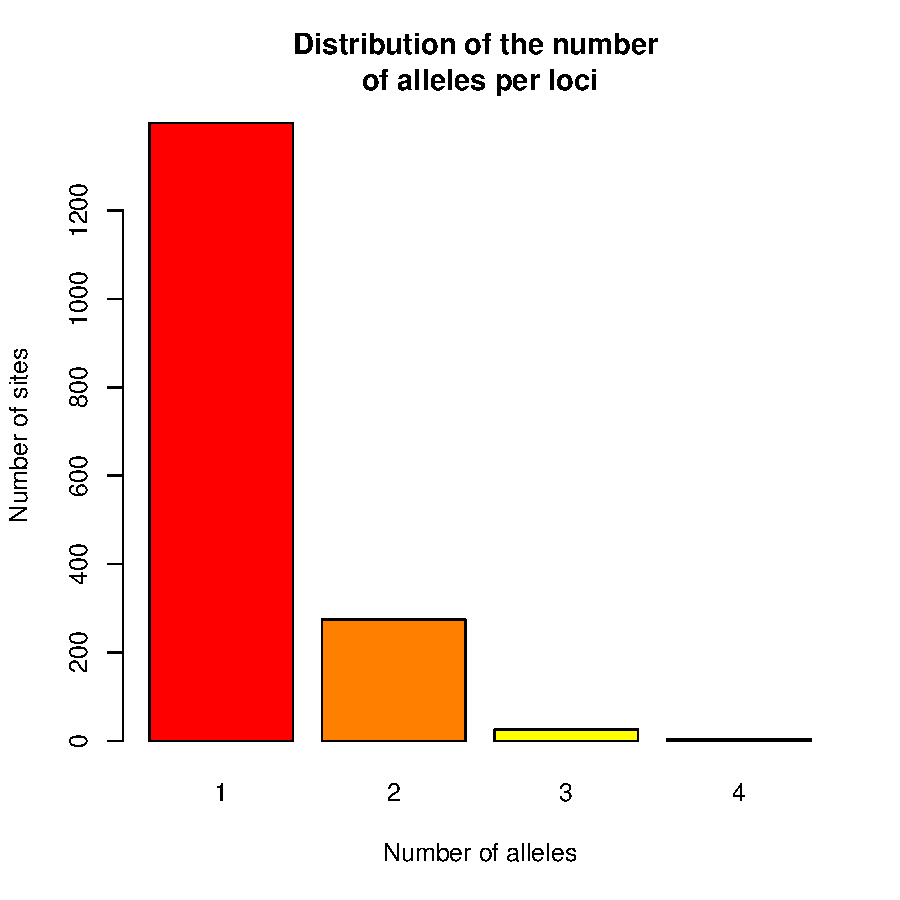
\includegraphics{figs/genomics-030}

\noindent Most polymorphic loci are biallelic, but a few loci with 3 or 4 alleles were lost.
We can estimate the loss of information very simply:
\begin{Schunk}
\begin{Sinput}
> temp <- temp[-1]
> temp <- 100 * temp/sum(temp)
> round(temp, 1)
\end{Sinput}
\begin{Soutput}
   2    3    4 
90.4  8.3  1.3 
\end{Soutput}
\end{Schunk}
In this case, 90.4\% of the polymorphic sites were biallelic, the others being
essentially triallelic.
This is probably a fairly exceptional situation due to the high mutation rate of the HA segment.







%%%%%%%%%%%%%%%%
%%%%%%%%%%%%%%%%
\section{Data analysis using \texttt{genlight} objects}
%%%%%%%%%%%%%%%%
%%%%%%%%%%%%%%%%

In the following, we illustrate some methods for the analysis of \texttt{genlight} objects, ranging
from simple tools for diagnosing allele frequencies or missing data to recently developed multivariate approaches.
Some examples below are illustrated using toy datasets generated using the function \texttt{glSim}.
This simple simulation tool allows for simulating large SNPs data with possibly contrasted
structures between two groups of individuals or patterns of linkage disequilibrium (LD).
See \texttt{?glSim} for more details on this tool.


%%%%%%%%%%%%%%%%
\subsection{Basic analyses}
%%%%%%%%%%%%%%%%


% % % % % % % % % %
\subsubsection{Plotting \texttt{genlight} objects}
% % % % % % % % % %
Basic features of the data may also be inferred by simply looking at the data.
\texttt{genlight} objects can be plotted using \texttt{glPlot}, or simply \texttt{plot} (both names
actually correspond to the same function).
This function displays the data as images, representing numbers of second alleles using colours.
For instance, we can have a feel for the amount and location of missing data in the influenza
dataset (see previous section) fairly easily:
\begin{Schunk}
\begin{Sinput}
> glPlot(flu, posi = "topleft")
\end{Sinput}
\end{Schunk}
The white streches in the first 30 SNPs observed around individual 70 indicate missing data.
There are only a few missing data, and they only concern a couple of individuals.
\\

In some simple cases, some biological structures might also be apparent in such plot.
For instance, we can generate data with independent SNPs distributions for two groups:
\begin{Schunk}
\begin{Sinput}
> x <- glSim(100, 0, 100, ploidy = 2)
\end{Sinput}
\end{Schunk}
\begin{Schunk}
\begin{Sinput}
> plot(x)
\end{Sinput}
\end{Schunk}
\begin{center}
  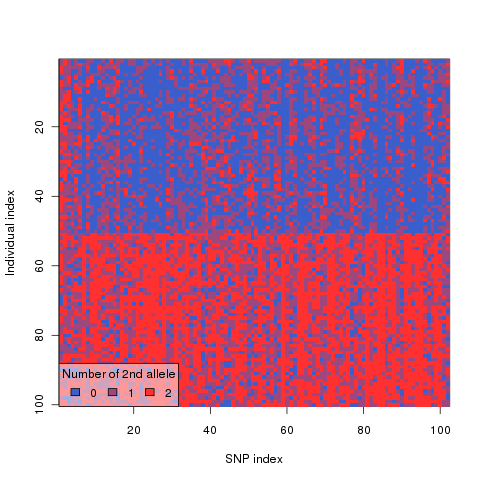
\includegraphics{figs/glsim1}
\end{center}

Strong patterns of LD between contiguous sites are also very easy to spot:
\begin{Schunk}
\begin{Sinput}
> x <- glSim(100, 100, ploidy = 2, LD = TRUE, block.size = 10)
\end{Sinput}
\end{Schunk}
\begin{Schunk}
\begin{Sinput}
> plot(x)
\end{Sinput}
\end{Schunk}
\begin{center}
  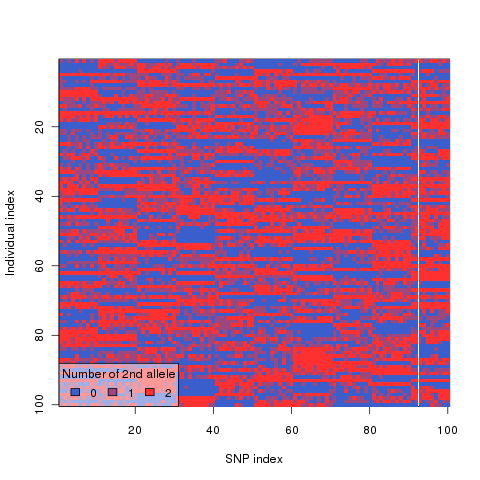
\includegraphics{figs/glsim2}
\end{center}

Of course, this is merely a very preliminary approach to the data.
More detailed analysis can be achieved using both standard and \textit{ad hoc} procedures as
detailed below.



% % % % % % % % % %
\subsubsection{\texttt{genlight}-optimized routines}
% % % % % % % % % %


Some simple operations such as computing allele frequencies or diagnosing missing values can be
problematic when the data matrix cannot be represented in memory.
\textit{adegenet} implements a few basic procedures which perform such basic tasks on
\texttt{genlight} objects processing one individual at a time, thereby minimizing memory
requirements. The most computer-intensive of these procedures can also use compiled C code and/or
multicore capabilities (when available) to speed up computations.
\\


All these procedures are named using the prefix \texttt{gl} (for \texttt{genlight}), and can therefore be listed by
typing \texttt{gl} and pressing the TAB key twice.
They are (see \texttt{?glMean}):
\begin{itemize}
\item \texttt{glSum}: computes the sum of second alleles for each SNP.
\item \texttt{glNA}: computes the number of missing values in each locus.
\item \texttt{glMean}: computes the mean of second alleles, i.e. second allele frequencies for
  each SNP.
\item \texttt{glVar}: computes the variance of the second allele frequency for each SNP.
\item \texttt{glDotProd}: computes the dot products between all pairs of individuals, with
  possible centring and scaling.
\end{itemize}
For instance, one can easily derive the distributiong of allele frequencies using:
\begin{Schunk}
\begin{Sinput}
> myFreq <- glMean(flu)
> hist(myFreq, proba = TRUE, col = "gold", xlab = "Allele frequencies", 
+     main = "Distribution of (second) allele frequencies")
> temp <- density(myFreq)
> lines(temp$x, temp$y * 1.8, lwd = 3)
\end{Sinput}
\end{Schunk}
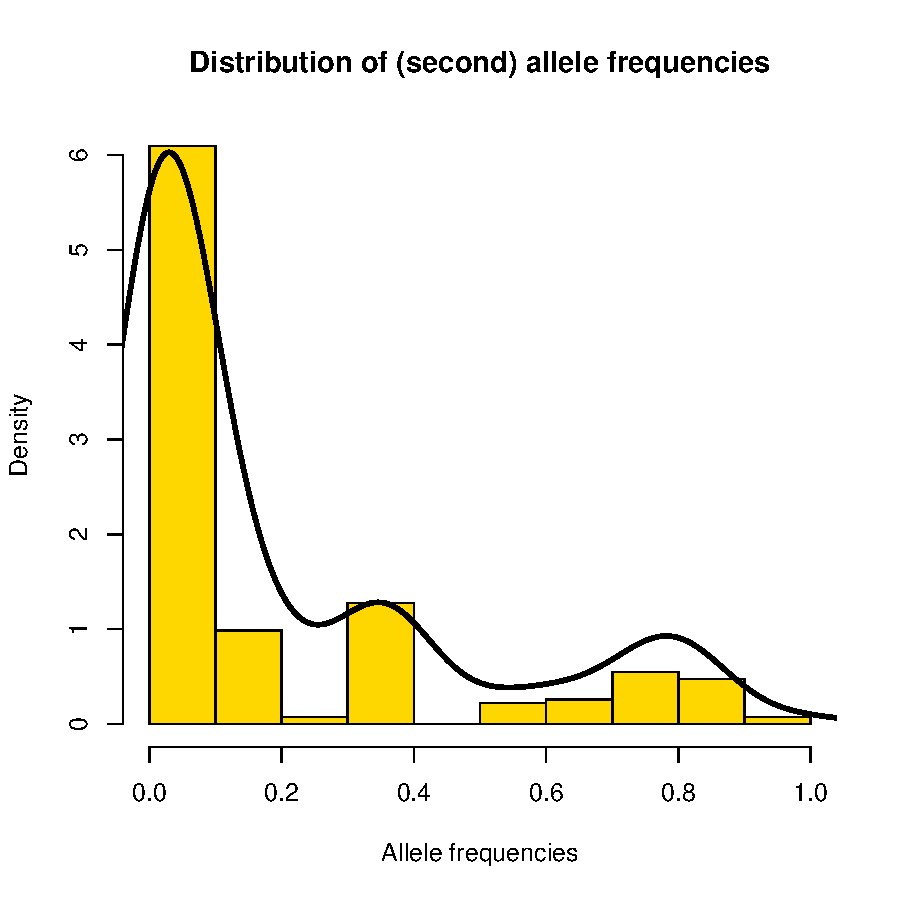
\includegraphics{figs/genomics-037}

\noindent In biallelic loci, one allele is always entirely redundant with the other, so it is generally
sufficient to analyse a single allele per loci.
However, the distribution of allele frequencies may be more interpretable by restoring its native symmetry:
\begin{Schunk}
\begin{Sinput}
> myFreq <- glMean(flu)
> myFreq <- c(myFreq, 1 - myFreq)
> hist(myFreq, proba = TRUE, col = "darkseagreen3", xlab = "Allele frequencies", 
+     main = "Distribution of allele frequencies", nclass = 20)
> temp <- density(myFreq, bw = 0.05)
> lines(temp$x, temp$y * 2, lwd = 3)
\end{Sinput}
\end{Schunk}
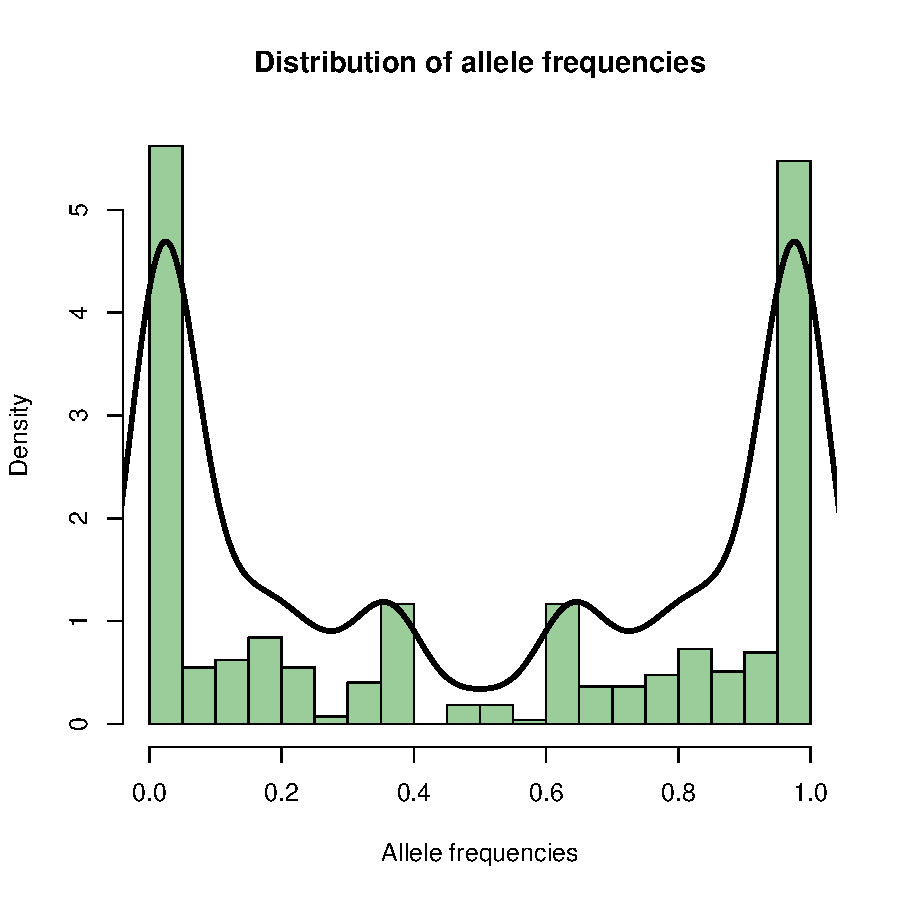
\includegraphics{figs/genomics-038}

\noindent While a large number of loci are nearly fixed (frequencies close to 0 or 1), there is an
appreciable number of alleles with intermediate frequencies and therefore susceptible to contain
interesting biological signal.
More generally and perhaps more importantly, this figure may also cast light on a well-known social
phenomenon occuring mainly in young people attending noisy kinds of conferences:
\begin{center}
  
\includegraphics{figs/devilsign}
\end{center}

\noindent We can indeed wonder whether the gesture usually referred to as the '\textit{devil sign}'
is not actually a reference to the usual shape of SNPs frequency distributions.  It is still
unclear, however, how many geneticists do attend metal gigs, although recent observations suggest
they would be more frequent in grindcore events than in classical heavy metal shows.
\\

Besides these considerations, we can also map missing data across loci as we have done for SNP positions in the
US influenza dataset (see previous section) using \texttt{glNA} and \texttt{density}:
\begin{Schunk}
\begin{Sinput}
> head(glNA(flu), 20)
\end{Sinput}
\begin{Soutput}
  7.a/g  12.c/t  31.t/c  32.t/c  36.t/c  37.c/a  44.t/c  45.c/t  52.a/g  60.c/t 
      2       2       2       2       2       2       2       2       1       1 
 62.g/t  72.c/a  73.a/g  78.a/g  96.a/g  99.c/t 105.a/g 108.g/a 121.c/a 128.a/g 
      1       1       1       1       1       1       0       0       0       0 
\end{Soutput}
\begin{Sinput}
> temp <- density(glNA(flu), bw = 10)
> plot(temp, type = "n", xlab = "Position in the alignment", main = "Location of the missing values (NAs)", 
+     xlim = c(0, 1701))
> polygon(c(temp$x, rev(temp$x)), c(temp$y, rep(0, length(temp$x))), 
+     col = transp("blue", 0.3))
> points(glNA(flu), rep(0, nLoc(flu)), pch = "|", col = "blue")
\end{Sinput}
\end{Schunk}

\noindent Here, the few missing values are all located at the beginning at the alignment, probably
reflecting heterogeneity in DNA amplification during the sequencing process.
In larger datasets, such simple investigation can give crucial insights about the quality of
the data and the existence of possible sequencing biases.
\\




% % % % % % % % % %
\subsubsection{Analysing data per block}
% % % % % % % % % %

Some operations such as computations of distances between individuals can also be useful,
and have yet to be implemented for \texttt{genlight} objects.
These operations are easy to carry out by converting data to alleles counts (using
\texttt{as.matrix}), but this conversion itself can be problematic because of memory limitations.
One easy workaround consists in parallelizing computations across blocks of loci.
\texttt{seploc} is first used to create a list of smaller \texttt{genlight} objects, each of which
can individually be converted to absolute allele frequencies using \texttt{as.matrix}.
Then, computations are carried on the list of object, without ever having to convert the entire
dataset, and results are finally reunited.
\\

Let us illustrate this procedure using 40 simulated individuals with 100,000 SNPs each:
\begin{Schunk}
\begin{Sinput}
> x <- glSim(40, 1e+05, LD = FALSE)
> x
\end{Sinput}
\begin{Soutput}
 === S4 class genlight ===
 40 genotypes,  100000 binary SNPs
 Ploidy: 1
 0 (0 %) missing data
 @pop: individual membership for 2 populations
\end{Soutput}
\end{Schunk}
\texttt{seploc} is used to create a list of smaller objects (here, 10 blocks of 10,000 SNPs):
\begin{Schunk}
\begin{Sinput}
> x <- seploc(x, n.block = 10)
> class(x)
\end{Sinput}
\begin{Soutput}
[1] "list"
\end{Soutput}
\begin{Sinput}
> names(x)
\end{Sinput}
\begin{Soutput}
 [1] "block.1"  "block.2"  "block.3"  "block.4"  "block.5"  "block.6" 
 [7] "block.7"  "block.8"  "block.9"  "block.10"
\end{Soutput}
\begin{Sinput}
> x[1:2]
\end{Sinput}
\begin{Soutput}
$block.1
 === S4 class genlight ===
 40 genotypes,  10000 binary SNPs
 Ploidy: 1
 0 (0 %) missing data
 @pop: individual membership for 2 populations

$block.2
 === S4 class genlight ===
 40 genotypes,  10000 binary SNPs
 Ploidy: 1
 0 (0 %) missing data
 @pop: individual membership for 2 populations
\end{Soutput}
\end{Schunk}
\texttt{dist} is used within a \texttt{lapply} loop to compute pairwise distances between
individuals for each block:
\begin{Schunk}
\begin{Sinput}
> lD <- lapply(x, function(e) dist(as.matrix(e)))
> class(lD)
\end{Sinput}
\begin{Soutput}
[1] "list"
\end{Soutput}
\begin{Sinput}
> names(lD)
\end{Sinput}
\begin{Soutput}
 [1] "block.1"  "block.2"  "block.3"  "block.4"  "block.5"  "block.6" 
 [7] "block.7"  "block.8"  "block.9"  "block.10"
\end{Soutput}
\begin{Sinput}
> class(lD[[1]])
\end{Sinput}
\begin{Soutput}
[1] "dist"
\end{Soutput}
\end{Schunk}
\texttt{lD} is a list of distances matrices (\texttt{dist} objects) between pairs of individuals.
The general distance matrix is obtained by summing these:
\begin{Schunk}
\begin{Sinput}
> D <- Reduce("+", lD)
\end{Sinput}
\end{Schunk}
And we could now carry on further analyses, such as a neighbor-joining tree using the \textit{ape} package:
\begin{Schunk}
\begin{Sinput}
> library(ape)
> plot(nj(D), type = "fan")
> title("A simple NJ tree of simulated genlight data")
\end{Sinput}
\end{Schunk}
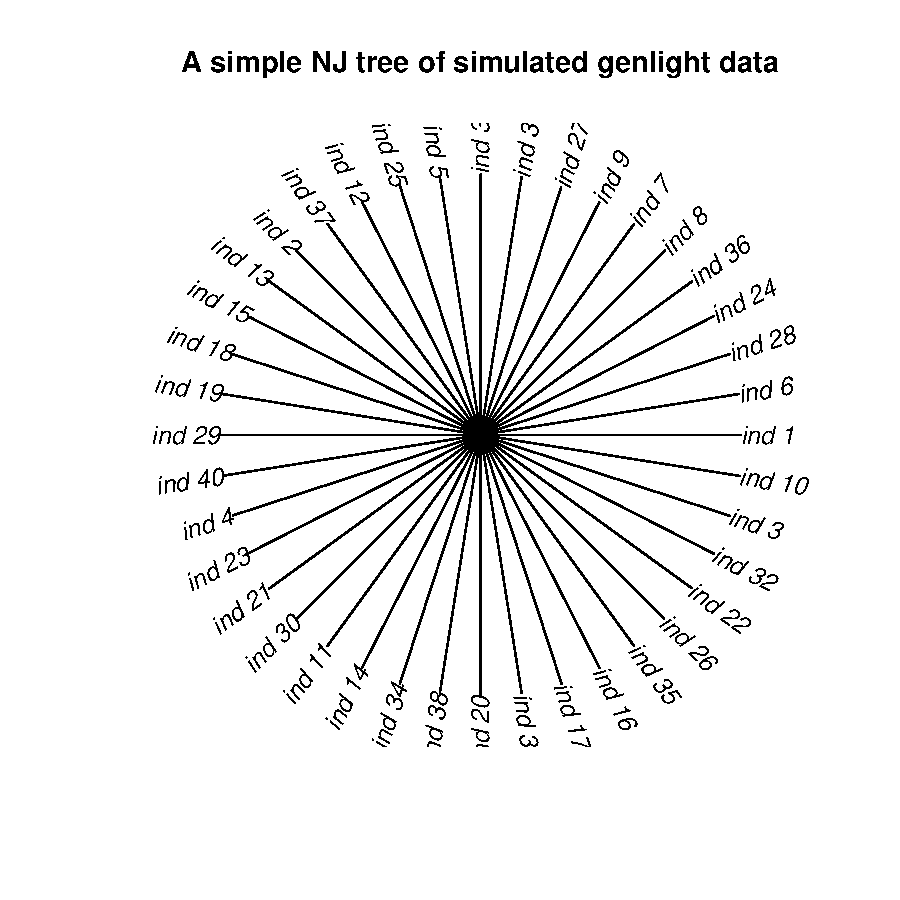
\includegraphics{figs/genomics-044}




% % % % % % % % % %
\subsubsection{What is the unit of observation?}
% % % % % % % % % %
Whenever ploidy varies across individuals, an issue arises as to what is defined as the \textit{unit of observation}.
Technically speaking, the unit of observation is the entity on which the observation is made.
When working with allelic data, it is not always clear what the unit of observation is.
The unit of observation may be:
\begin{itemize}
  \item \textit{individuals}: in this case each individual is represented by a vector of allele frequencies
  \item \textit{alleles}: in this case we consider that each individual represents a sample of
    alleles, with a sample size equalling the ploidy for each locus
\end{itemize}

This distinction is most of the time overlooked when analysing genetic data.
As a matter of fact, it does not matter when all individuals have the same ploidy.
For instance, if we take the following data:
\begin{Schunk}
\begin{Sinput}
> x <- new("genlight", list(a = c(0, 0, 1, 1), b = c(1, 1, 0, 0), 
+     c = c(1, 1, 1, 1)))
> locNames(x) <- 1:4
> x
\end{Sinput}
\begin{Soutput}
 === S4 class genlight ===
 3 genotypes,  4 binary SNPs
 Ploidy: 1
 0 (0 %) missing data
 @loc.names: labels of the SNPs
\end{Soutput}
\begin{Sinput}
> as.matrix(x)
\end{Sinput}
\begin{Soutput}
  1 2 3 4
a 0 0 1 1
b 1 1 0 0
c 1 1 1 1
\end{Soutput}
\end{Schunk}
and assume that all individuals are haploid, then computing e.g. the allele frequencies is
straightforward (they all equal $2/3$):
\begin{Schunk}
\begin{Sinput}
> glMean(x)
\end{Sinput}
\begin{Soutput}
        1         2         3         4 
0.6666667 0.6666667 0.6666667 0.6666667 
\end{Soutput}
\end{Schunk}
Let us no consider a sightly different case:
\begin{Schunk}
\begin{Sinput}
> x <- new("genlight", list(a = c(0, 0, 2, 2), b = c(1, 1, 0, 0), 
+     c = c(1, 1, 1, 1)))
> locNames(x) <- 1:4
> x
\end{Sinput}
\begin{Soutput}
 === S4 class genlight ===
 3 genotypes,  4 binary SNPs
 Ploidy statistics (min/median/max): 1 / 1 / 2
 0 (0 %) missing data
 @loc.names: labels of the SNPs
\end{Soutput}
\begin{Sinput}
> as.matrix(x)
\end{Sinput}
\begin{Soutput}
  1 2 3 4
a 0 0 2 2
b 1 1 0 0
c 1 1 1 1
\end{Soutput}
\begin{Sinput}
> ploidy(x)
\end{Sinput}
\begin{Soutput}
a b c 
2 1 1 
\end{Soutput}
\end{Schunk}
What are the allele frequencies in this case?
Well, it depends on what we mean by '\textit{allele frequency}'.
\\


Is it the frequency of the alleles in the population?
In this case, the unit of observation is the allele.
We have a total of 4 samples for each loci, (since '\texttt{a}' is diploid, it
represents actually two samples) and the frequencies are $1/2$, $1/2$, $3/4$, $3/4$.
Note, however, that this assumes that alleles are randomly associated within individuals (pangamy).

Or is it the frequency of the alleles within the individuals?
In this case, the unit of observation is the individual, and the vector of allele frequencies represents the 'average individual'.
We first need to convert each individual vector into relative frequencies (i.e., divide by their respective ploidy), and then compute the
average frequency across individuals, which ends up with $2/3$ for each locus:
\begin{Schunk}
\begin{Sinput}
> M <- as.matrix(x)/ploidy(x)
> apply(M, 2, mean)
\end{Sinput}
\begin{Soutput}
        1         2         3         4 
0.6666667 0.6666667 0.6666667 0.6666667 
\end{Soutput}
\end{Schunk}

The procedures designed for \texttt{genlight} objects seen above (\texttt{glMean}, \texttt{glNA},
etc.) allow for this distinction to be made.
The option \texttt{alleleAsUnit} is a logical indicating whether the observation unit is the allele
(\texttt{TRUE}, default) or the individual (\texttt{FALSE}).
For instance:
\begin{Schunk}
\begin{Sinput}
> as.matrix(x)
\end{Sinput}
\begin{Soutput}
  1 2 3 4
a 0 0 2 2
b 1 1 0 0
c 1 1 1 1
\end{Soutput}
\begin{Sinput}
> glMean(x, alleleAsUnit = TRUE)
\end{Sinput}
\begin{Soutput}
   1    2    3    4 
0.50 0.50 0.75 0.75 
\end{Soutput}
\begin{Sinput}
> glMean(x, alleleAsUnit = FALSE)
\end{Sinput}
\begin{Soutput}
        1         2         3         4 
0.6666667 0.6666667 0.6666667 0.6666667 
\end{Soutput}
\end{Schunk}





%%%%%%%%%%%%%%%%
\subsection{Principal Component Analysis (PCA)}
%%%%%%%%%%%%%%%%
Principal Component Analysis (PCA) is implemented for \texttt{genlight} objects by the function \texttt{glPca}.
This function can accommodate any level of ploidy in the data (including varying ploidy across
individuals). More importantly, it performs computations without ever processing more than a
couple of genomes at a time, thereby minimizing memory requirements.
It also uses compiled C code and possibly multicore ressources if available to speed up computations.
We illustrate the method on the previously introduced influenza dataset (object \texttt{flu}):
\begin{Schunk}
\begin{Sinput}
> flu
> pca1 <- glPca(flu)
\end{Sinput}
\end{Schunk}
\begin{center}
  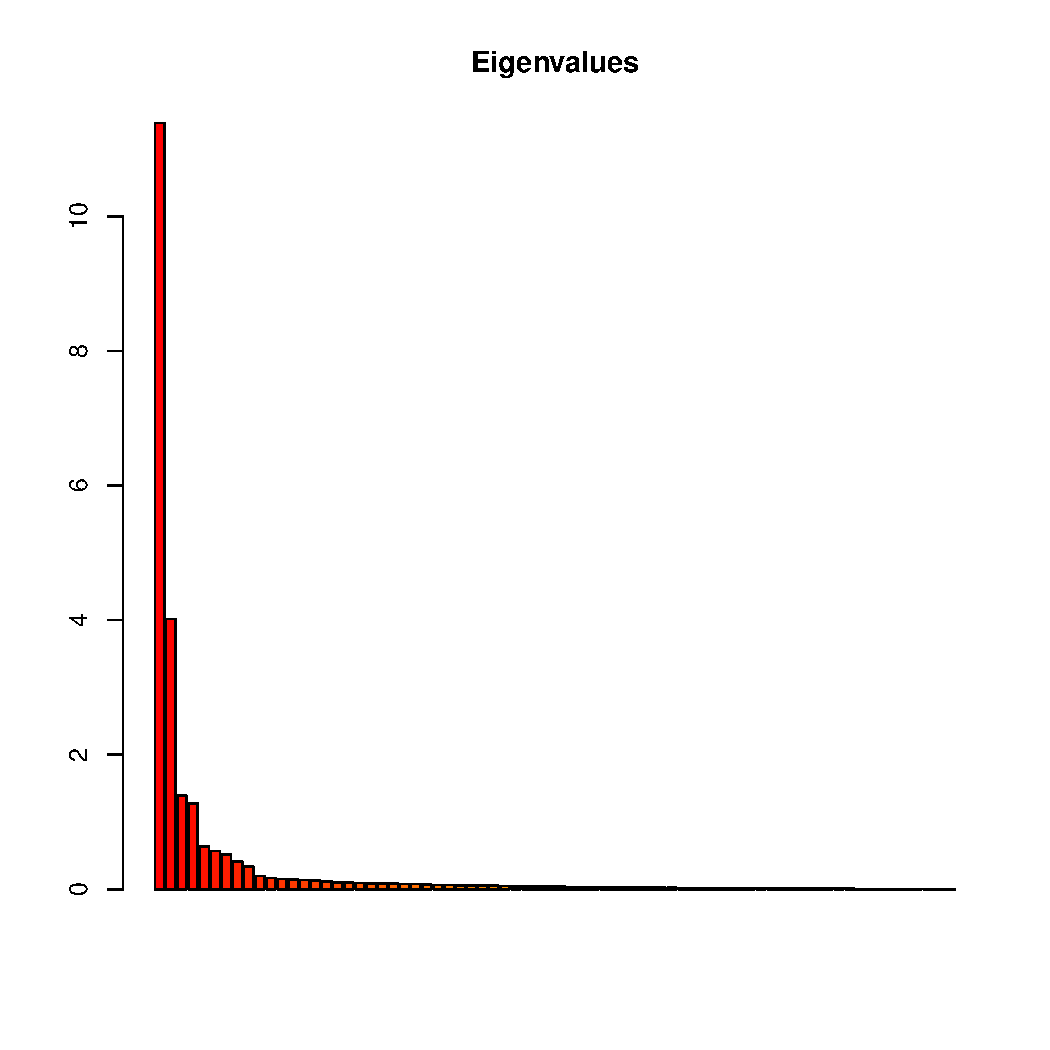
\includegraphics{figs/pca1}
\end{center}
When \texttt{nf} (number of retained factors) is not specified, the function displays the barplot of
eigenvalues of the analysis and asks the user for a number of retained principal components.
\texttt{glPca} returns a list with the class \texttt{glPca} containing the eigenvalues, principal
components and loadings of the analysis:
\begin{Schunk}
\begin{Sinput}
> pca1
\end{Sinput}
\begin{Soutput}
 === PCA of genlight object ===
Class: list of type glPca
Call ($call):glPca(x = flu)

Eigenvalues ($eig):
 11.385 4.019 1.391 1.275 0.636 0.569 ...

Principal components ($scores):
 matrix with 80 rows (individuals) and 4 columns (axes) 

Principal axes ($loadings):
 matrix with 274 rows (SNPs) and 4 columns (axes) 
\end{Soutput}
\end{Schunk}

In addition to usual graphics, \texttt{glPca} object can displayed using \texttt{scatter} (produces
a scatterplot of the principal components (PCs)) and \texttt{loadingplot} (plots the allele contributions,
i.e. squared loadings).
The scatterplot is obtained by:
\begin{Schunk}
\begin{Sinput}
> scatter(pca1, posi = "bottomright")
> title("PCA of the US influenza data\n axes 1-2")
\end{Sinput}
\end{Schunk}
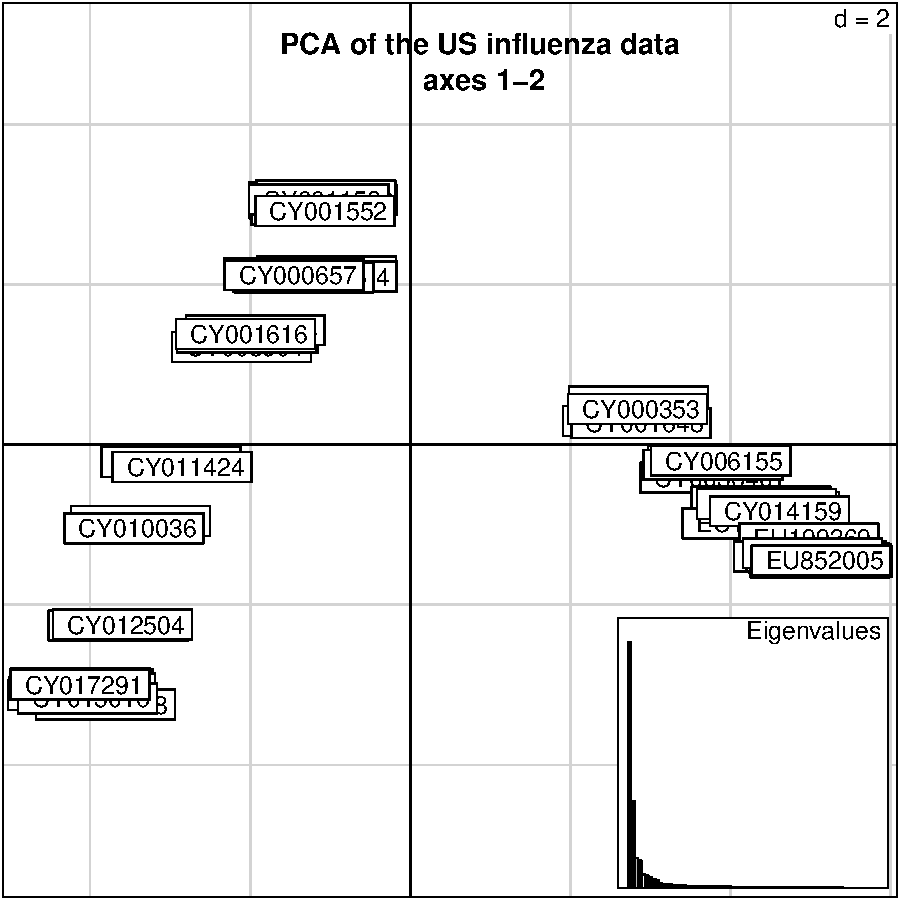
\includegraphics{figs/genomics-053}
The first PC suggests the existence of two clades in the data, while the second one shows groups of
closely related isolates arranged along a cline of genetic differentiation.
This structure is confirmed by a simple neighbour-joining (NJ) tree:
\begin{Schunk}
\begin{Sinput}
> library(ape)
> tre <- nj(dist(as.matrix(flu)))
> tre
\end{Sinput}
\begin{Soutput}
Phylogenetic tree with 80 tips and 78 internal nodes.

Tip labels:
	 CY013200,  CY013781,  CY012128,  CY013613,  CY012160,  CY012272, ...

Unrooted; includes branch lengths.
\end{Soutput}
\begin{Sinput}
> plot(tre, typ = "fan", cex = 0.7)
> title("NJ tree of the US influenza data")
\end{Sinput}
\end{Schunk}

The correspondance between both analyses can be better assessed using colors based on PCs; this is
achieved by \texttt{colorplot}:
\begin{Schunk}
\begin{Sinput}
> myCol <- colorplot(pca1$scores, pca1$scores, transp = TRUE, cex = 4)
> abline(h = 0, v = 0, col = "grey")
> add.scatter.eig(pca1$eig[1:40], 2, 1, 2, posi = "topright", inset = 0.05, 
+     ratio = 0.3)
\end{Sinput}
\end{Schunk}
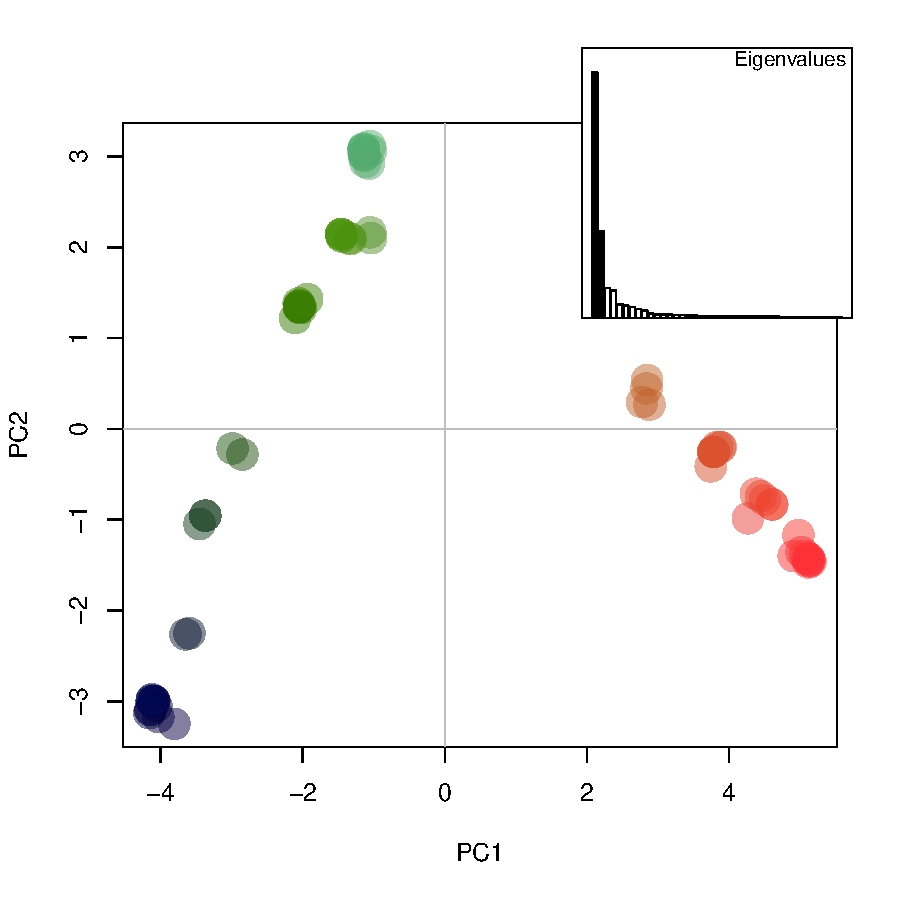
\includegraphics{figs/genomics-055}

\begin{Schunk}
\begin{Sinput}
> plot(tre, typ = "fan", show.tip = FALSE)
> tiplabels(pch = 20, col = myCol, cex = 4)
> title("NJ tree of the US influenza data")
\end{Sinput}
\end{Schunk}
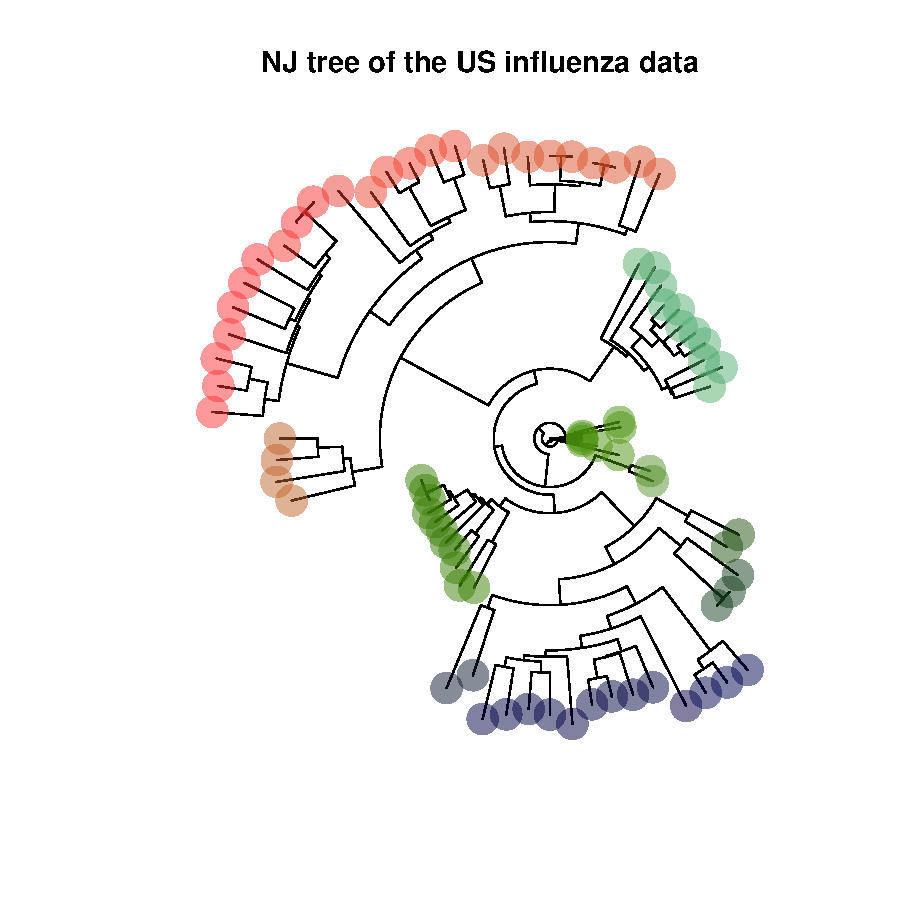
\includegraphics{figs/genomics-056}

\noindent As expected, both approaches give congruent results, but both are complementary: NJ is
better at showing bunches of related isolates, but the cline of genetic differentiation is much
clearer in PCA.




%%%%%%%%%%%%%%%%
\subsection{Discriminant Analysis of Principal Components (DAPC)}
%%%%%%%%%%%%%%%%
Discriminant analysis of Principal Components (DAPC) is implemented for \texttt{genlight} objects by
an appropriate method for the \texttt{find.clusters} and \texttt{dapc} generics.
To put it simply, you can run \texttt{find.clusters} and \texttt{dapc} on \texttt{genlight} objects and the appropriate
functions will be used.
As in \texttt{glPca}, these methods never require more than a couple of genomes to be translated into
allele frequencies at a time, thereby minimizing RAM requirements.
\\

Below, we illustrate DAPC on a \texttt{genlight} including only 50 structured SNPs out of 50,000
non-structured SNPs:
\begin{Schunk}
\begin{Sinput}
> x <- glSim(100, 50000, 50)
> x
\end{Sinput}
\begin{Soutput}
 === S4 class genlight ===
 100 genotypes,  50050 binary SNPs
 Ploidy: 1
 0 (0 %) missing data
 @pop: individual membership for 2 populations
\end{Soutput}
\begin{Sinput}
> dapc1 <- dapc(x, n.pca = 20, n.da = 1)
\end{Sinput}
\end{Schunk}

For the last 50 structured SNPs (located at the end of the alignment), the two groups of individuals have different (random) distribution of
allele frequencies, while they share the same distributions in other loci.
DAPC can still make some decent discrimination:
\begin{Schunk}
\begin{Sinput}
> scatter(dapc1, scree.da = FALSE, bg = "white", posi.pca = "topright", 
+     legen = TRUE, txt.leg = paste("group", 1:2), col = c("red", 
+         "blue"))
\end{Sinput}
\end{Schunk}
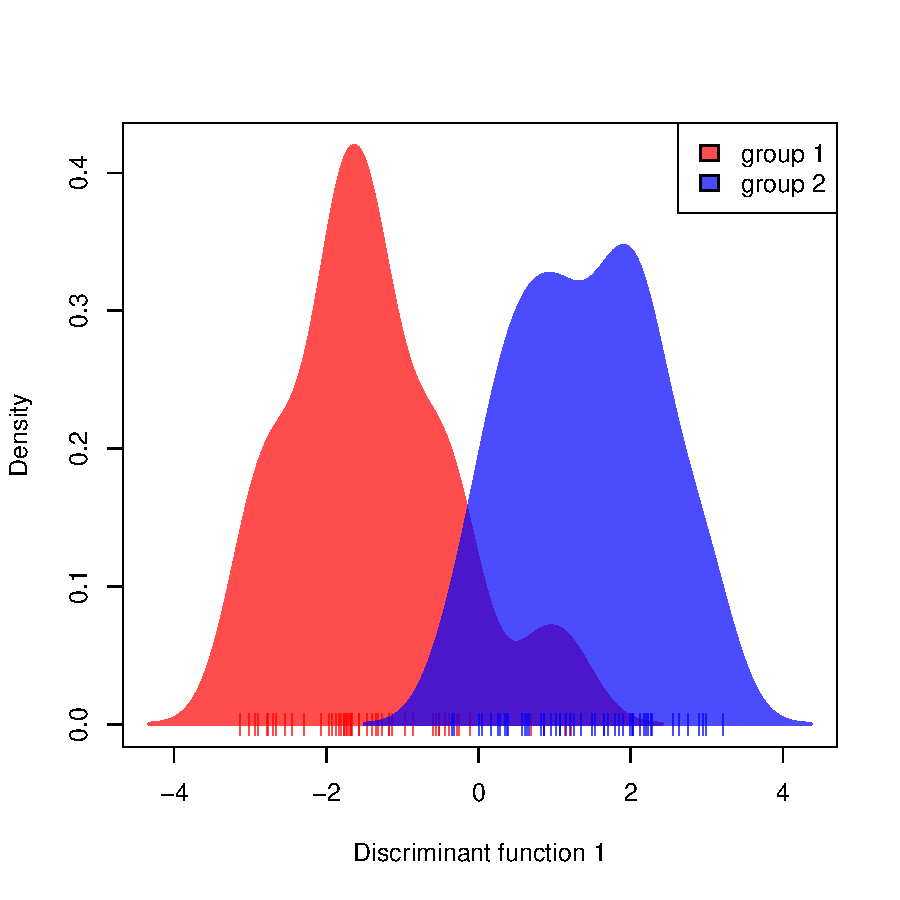
\includegraphics{figs/genomics-058}

\noindent While the composition plot confirms that groups are not entirely disentangled...
\begin{Schunk}
\begin{Sinput}
> compoplot(dapc1, col = c("red", "blue"), lab = "", txt.leg = paste("group", 
+     1:2), ncol = 2)
\end{Sinput}
\end{Schunk}
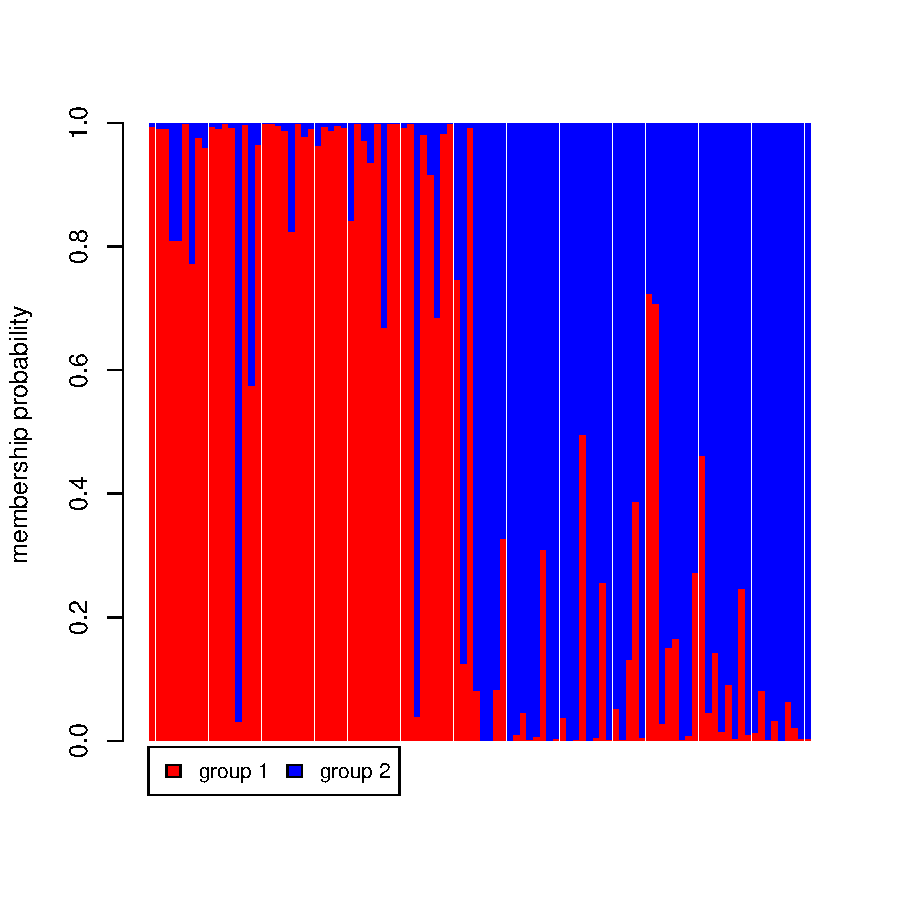
\includegraphics{figs/genomics-059}

\noindent ... the loading plot identifies pretty well the most discriminating alleles:
\begin{Schunk}
\begin{Sinput}
> loadingplot(dapc1$var.contr, thres = 4e-04)
\end{Sinput}
\end{Schunk}

\begin{center}
  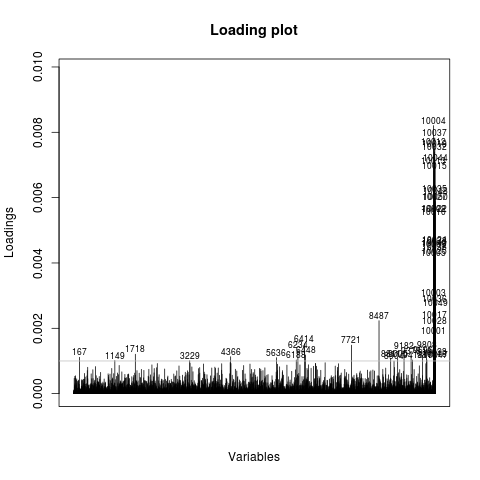
\includegraphics{figs/loadingplotGL}
\end{center}

\noindent And we can zoom in to the contributions of the last 100 SNPs to make sure that the tail indeed
corresponds to the 50 last structured loci:
\begin{Schunk}
\begin{Sinput}
> loadingplot(tail(dapc1$var.contr[, 1], 100))
\end{Sinput}
\end{Schunk}
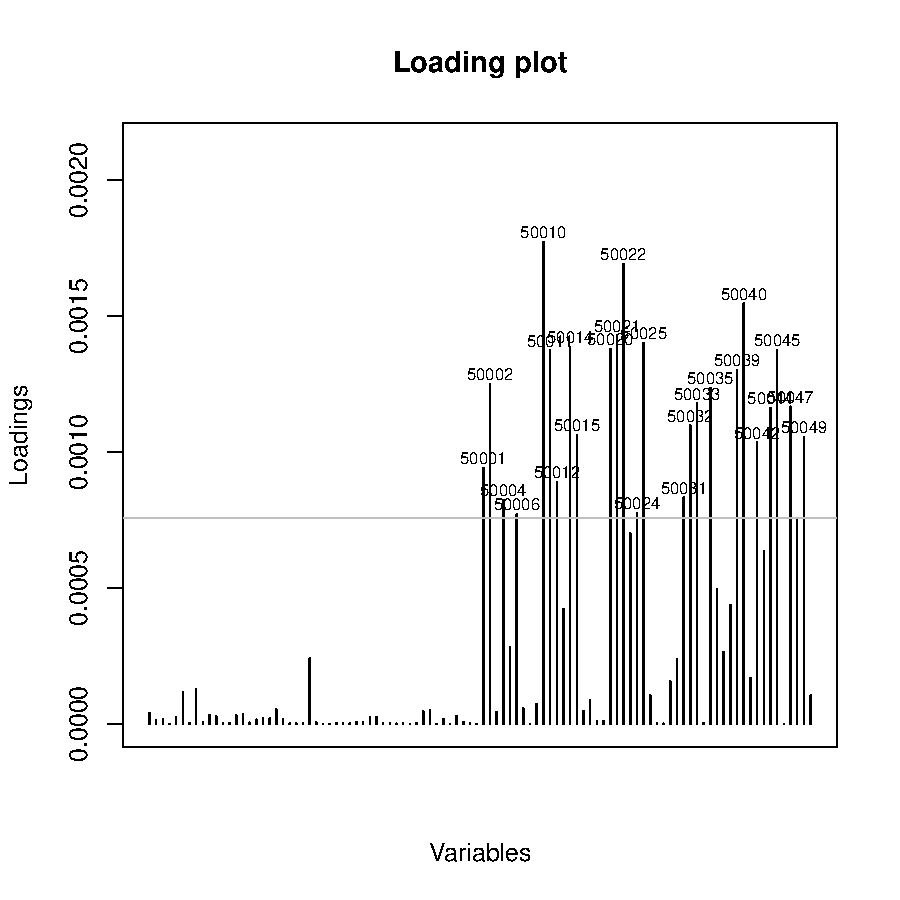
\includegraphics{figs/genomics-061}

\noindent Here, we indeed identified the structured region of the genome fairly well.







\begin{thebibliography}{9}

\bibitem{tjart05}
  Jombart, T. (2008) adegenet: a R package for the multivariate
  analysis of genetic markers. \textit{Bioinformatics} 24: 1403-1405.

\bibitem{np145}
  R Development Core Team (2011). R: A language and environment for
  statistical computing. R Foundation for Statistical Computing,
  Vienna, Austria. ISBN 3-900051-07-0.

\end{thebibliography}


\end{document}
